% !TEX encoding = UTF-8 Unicode
% !TEX TS-program = XeLaTex


\documentclass[8pt, twoside, a5paper]{extreport}
\usepackage{lipsum} % ----------------------------------------------------------- cancellabile
\usepackage{blindtext}	% dummy text

\usepackage{latexsym}
\usepackage[polutonikogreek, italian, english]{babel}
\usepackage[T1]{fontenc}
%\usepackage[utf8]{inputenc}

\usepackage[margin=1cm]{geometry}

\usepackage{multicol}
\usepackage[hang, small,labelfont=bf,up,textfont=it,up]{caption} % Custom captions under/above floats in tables or figures
\usepackage{booktabs} % Horizontal rules in tables
\usepackage{float} % they need to be placed in specific locations with the [H] (e.g. \begin{table}[H])

\usepackage{afterpage}

\usepackage{graphicx}
\usepackage{amssymb}
\usepackage{epstopdf}

\usepackage{pst-barcode}

\usepackage{hyperref} % For hyperlinks in the PDF

\usepackage{titlesec} % Allows customization of titles
\renewcommand\thesection{\Roman{section}} % Roman numerals for the sections
\renewcommand\thesubsection{\Roman{subsection}} % Roman numerals for subsections
\titleformat{\section}[block]{\large\scshape\centering}{\thesection.}{1em}{} % Change the look of the section titles
\titleformat{\subsection}[block]{\large}{\thesubsection.}{1em}{} % Change the look of the section titles

% \usepackage{fancyhdr} % Headers and footers
% \pagestyle{fancy} % All pages have headers and footers
% \fancyhead{} % Blank out the default header
% \fancyfoot{} % Blank out the default footer
% \fancyhead{}%[C]{Sei volte EMUfest $\bullet$ Novembre 2013 }%$\bullet$ Vol. XXI, No. 1} % Custom header text
% \fancyfoot[RO,LE]{\thepage} % Custom footer text

\renewcommand{\thefootnote}{\textasteriskcentered}

\usepackage{mwe,tikz}
\usepackage{tcolorbox}

\usepackage{color}

\usepackage{fontspec,xltxtra,xunicode}
\defaultfontfeatures{Mapping=tex-text}
\setromanfont[Mapping=tex-text]{Source Sans Pro}
\setsansfont[Scale=MatchLowercase,Mapping=tex-text]{Source Sans Pro}
\setmonofont[]{Source Code Pro}

\newfontfamily{\svolk}{Volkhov}

\linespread{1.03}

\usepackage{lipsum}

\definecolor{supercolor}{RGB}{3,39,36}

%\topmargin -2.66in

\newtcbox{\mybox}{nobeforeafter,colframe=supercolor,colback=supercolor,boxrule=0.5pt,arc=8pt,
  boxsep=0pt,left=2pt,right=2pt,top=6pt,bottom=2pt,tcbox raise base}

\newcommand\blankpage{%
    \null
    \thispagestyle{empty}%
    \addtocounter{page}{-1}%
    \newpage}

% !TEX encoding = UTF-8 Unicode
% !TEX TS-program = XeLaTex
% !TEX root = EMU2015_booklet.tex

%----------------------------------------------------------------------------------------
%	NEW COMMANDS 2015
%----------------------------------------------------------------------------------------

\newcommand{\greco}[1]{%
\begin{otherlanguage*}{greek}#1\end{otherlanguage*}}


%----------------------------------------------------------------------------------------
\newcommand{\livel}[6]{%
\noindent \textsc{#1}\\ %
\noindent \textbf{\textit{#2}} -- #3\\%
\noindent #4\\ %
\noindent #5 -- \textsc{#6}%
\\
}%

%: #1 autore, #2 titolo, #3 anno ed esecuzione, #4 tipologia, #5 strumenti, #6 esecutori

%\livel{}
%{}{}
%{}
%{}{}


%-----------------------------------------------------------------------------------------------------------------
\newcommand{\acusmatico}[4]{%
\noindent \textsc{#1}\\ %
\noindent \textbf{\textit{#2}} -- #3\\%
\noindent #4%
\\
}%

%: #1 autore, #2 titolo, #3 anno ed esecuzione, #4 tipologia
%\acusmatico{}
%{}{}
%{}

%-----------------------------------------------------------------------------------------------------------------
\newcommand{\acusmatici}[3]{%
\noindent \textsc{#1}\\ %
\noindent \textbf{\textit{#2}} -- #3%
\\
}%

%: #1 autore, #2 titolo, #3 anno ed esecuzione
%\acusmatici{}
%{}{}


%-----------------------------------------------------------------------------------------------------------------
\newcommand{\descrizione}[2]{%
\noindent \textbf{\textit{#1}} %
#2 %
\\
}%

%: #1 titolo, #2 abstract
% \descrizione{}{}


%-----------------------------------------------------------------------------------------------------------------
\newcommand{\biografia}[2]{%
\noindent \textsc{#1} %
#2 %
\medskip
}%

%: #1 autore, #2 biografia
% \biografia{}{}



%----------------------------------------------------------------------------------------
%	TITLE SECTION
%----------------------------------------------------------------------------------------

\title{
	\svolk{CONSERVATORIO DI MUSICA S. CECILIA} \\
	%\vspace{-15mm}
	\fontsize{50}{50}
	\svolk{
		\emph{
			EMUFest 2015
			}
		}
	} % Article title

\author{
	\textsc{Conservatorio di Musica Santa Cecilia} \\
	5 -- 10 ottobre 2015 \\
	\textsc{Università di Roma Tor Vergata} \\
	13 e 14 ottobre 2015 \\
	Roma
}

\vfill

\date{}

%\dedica{.2\textwidth}{\small A Monica:\\
%per tutto ciò che mi hai insegnato\\
%e per tutto ciò che ancora avresti dovuto insegnarmi.}

%----------------------------------------------------------------------------------------

\begin{document}
\pagestyle{empty}
\maketitle 

\afterpage{\blankpage}

\clearpage

~\vfill

% !TEX encoding = UTF-8 Unicode
% !TEX TS-program = XeLaTex
% !TEX root = EMU2015_booklet.tex

{\fontsize{30}{30} \svolk{\emph{Passare all'atto}}}

% \svolk{\emph{Passer à l’acte)}

\begin{quote}
\begin{it}
	\svolk{Il programma EMUfest 2015 ricava dalle suggestioni del titolo il criterio
di selezione delle opere e  intende offrire al pubblico una panoramica
delle attuali esperienze compositive: quelle che nascono dalla ricerca,
dalla scoperta, dall’invenzione.

Nessuna pratica artistica è fine solo a se stessa e anche la musica,
astratta e immateriale, porta in se questa responsabilità. L’idea è ciò che
il compositore incarna nella musica ma è pure la conseguenza di una
interpretazione della realtà, una visione dei valori o delle derive della
nostra civiltà.

L’elemento essenziale che permette ad un’opera d’arte di compiersi e di
trasmettere i suoi contenuti  è la correlazione tra la necessità interiore
dell’artista e la scelta del modo di esprimerla. \emph{Passer à l’acte} è
dunque il gesto che definisce la pratica artistica ma, allo stesso tempo e
in modo indiretto, è anche l’esortazione per noi fruitori, a cogliere gli
stimoli offerti dall’opera e a rendere attiva la nostra riflessione.}

\hfill \emph{Michelangelo Lupone}

\end{it}
\end{quote}

\clearpage

%----------------------------------------------------------------------------------------


\clearpage
%----------------------------------------------------------------------------------------

\section*{13 ottobre 2015 -- ore 18:00}

\subsection*{{\small Concerto Acusmatico \& Live Electronics\footnote{ Il concerto verrà trasmesso in diretta streaming da Radio Cemat}} \\
	\textsf{Auditorium Ennio Morricone}}

{\fontsize{30}{30} \svolk{\emph{ATTO XI}}}

\subsection*{\textsf{Regia del suono di Massimiliano Mascaro}}

\begin{quote}

{\svolk \small
\begin{quote}Vieni, disse la Musa,\\
cantami un canto che nessun poeta ha mai cantato,\\
cantami l'universale.\\
Nella nostra vasta terra,\\
in mezzo alla volgarità smisurata e alla feccia,\\
racchiuso e sicuro nel suo cuore più intimo,\\
si nasconde il seme della perfezione.\\
\hspace{1mm}\emph{Walt Whitman - Canto dell'universale}
\end{quote}

\begin{quote}«La metafora è probabilmente la forza più feconda che l'uomo possieda.»\\
\hspace{1mm}\emph{Jos\'e Ortega y  Gasset - La disumanizzazione dell'arte}
\end{quote}

L'esibizione Atto XI racchiude cinque brani che inglobano le varie forme della musica elettronica, passando da un live-electronics a un acustico e tape, finendo con un acusmatico. I titoli di questi lavori hanno come filo conduttore il rapporto tra l'ambiente e la natura umana che li integra e li unisce.}

\emph{M. Mascaro}
\end{quote}    


\vspace{3mm}

\begin{multicols}{2}

% !TEX encoding = UTF-8 Unicode
% !TEX TS-program = XeLaTex
% !TEX root = EMU2015_booklet.tex

\livel{Frei}
{Poetics}{16'50''}
{per due laptop}
{2015}

\livel{Christian Banasik}
{Ik ́}{9'}
{per flauto e live electronics}
{2013}

\livel{Marco Marinoni}
{Finita è la terra}{4'16''} %
{pianoforte e live electronics}
{2015}

\livel{Domenico De Simone}
{A[LIVE]}{5'30''}
{pianoforte, vibrafono  ed elettronica su supporto}
{2015}

\brano{Benjamin D. Whiting}
{Illumina! Arabidopsis thaliana}{9'18''}
{acusmatico}{2015}\\

\esecutore{flauto}{Elena D'Alò}
\esecutore{pianoforte}{Sara Ferrandino}
\esecutore{vibrafono}{Matteo Rossi}

\noindent \textsc{Frei}:\\
\esecutore{due laptop}{Francesco Bianco, Paolo Gatti}

% \descrizione{Poetics}{Work based on the concepts of entropy, redundancy, and noise and how these play a role on messages and information in a musical discourse. From an aesthetic point of view, everything is resolved, here, in an alternation between punctiform moments, almost static, and growing dynamic more or less sudden.}

\descrizione{Poetics}{Lavoro basato sull'improvvisazione giocata sull'alternanza fra momenti puntiformi, quasi statici, e dinamiche di crescendo più o meno improvvise. Altro tema trattato è il rapporto fra comunicabilità e incomunicabilità tramite l'indagare delle modalità di trasmissione dei messaggi musicali e vocali e i concetti di entropia, ridondanza e di rumore.}

% \descrizione{Ik ́}{\textit{Ik ́} is the name of the 2nd day in the ritual calendar of the Maya associated with breath and wind.The liturgical year consisted of twenty cycles and their glyphs, each of them thirteen days long, and had 260 days in all. For the tone material I use a contemporary folk song from Central America and a virtually generated original song of the Maya.The flute score consists of virtuoso abstracted variations mixed with the graphical-audio analysis of this particular glyph. It is divided in 20 parts.}

\descrizione{Ik ́}{\textit{Ik ́} è il nome del secondo giorno del calendario rituale dei Maya, associato al respiro e al vento. L'anno liturgico era composto da venti cicli e i loro glifi, ognuno dei quali durava tredici giorni, avendo in totale 260 giorni. Per il materiale tonale ho usato una canzone popolare contemporanea dell'America Centrale, e una canzone dei Maya generata virtualmente. La parte del flauto consiste in variazioni astratte miste all'analisi grafica-audio di questo particolare glifo. È diviso in 20 parti.}

% \descrizione{Finita è la terra}{is a small formal experiment that makes use of three piano sound objects, variants of a single musical image, which remain identical to themselves during the entire piece, arranged in a formal course partly iterative and partly structured through microvariations. These objects interact along the time axis with material fixed on support, agglomerations deriving from their possible electroacoustic processing – a live-electronics frozen, or even more than a live-electronics, an image of it, captured and distilled through an alchemical process which aims to turn something that was only movement, dispersion, probability (grain clouds applied to the three sound events of origin) in its \greco{εἴδωλον}, playing this way with the perception and memory in a continuum consisting of appearance / disappearance / memory / expectation / desire.}

\descrizione{Finita è la terra}{è un piccolo esperimento formale che fa uso di tre oggetti sonori pianistici, varianti di un'unica immagine musicale, che permangono identici a se stessi durante tutto il brano, disposti secondo un decorso formale in parte iterativo e in parte microvariato. Tali oggetti interagiscono lungo l’asse del tempo con materiali fissati su supporto, agglomerazioni derivanti da una loro possibile processazione elettroacustica – un live-electronics ghiacciato, o ancora, più che un live-electronics, una sua immagine, catturata e distillata, mediante un processo alchemico volto a trasformare qualcosa che era solo movimento, dispersione, probabilità (le nubi di granulazioni applicate ai tre eventi sonori di partenza) nel suo \greco{εἴδωλον}, giocando in questo modo con la percezione e la memoria in un continuum fatto di apparizione/sparizione/ricordo/attesa / desiderio.}

% \descrizione{A[LIVE]}{I AM NOT THERE \\ Do not stand at my grave and weep. \\ I am not there. I do not sleep. \\ I am a thousand winds that blow. \\ I am the diamond glints on snow. \\ I am the sunlight on ripened grain.  \\ I am the gentle autumn rain. \\ When you awaken in the morning’s hush \\ I am the swift uplifting rush \\ Of quiet birds in circled flight. \\ I am the soft stars that shine at night. \\ Do not stand at my grave and cry; \\ I am not there. I did not die. \\ Mary Elizabeth Frye}

\descrizione{A[LIVE]}{IO NON SONO LÌ \\ Non piangere sulla mia tomba.  \\ Io non sono lì. Io non sto dormendo.  \\ Io sono mille venti che soffiano. \\ Sono lo scintillio del diamante sulla neve. \\ Sono il sole che brilla sul grano maturo. \\ Sono la lieve pioggia d'autunno.  \\ Quando tu ti svegli nel silenzio del mattino, \\ io sono il rapido fruscio \\  degli uccelli che volano in cerchio. \\ Io sono la piccola stella che brilla di notte. \\ Non piangere sulla mia tomba;  \\ io non sono lì, la mia anima non è morta.   \\ (libera traduzione della poesia I AM NOT THERE di Mary Elizabeth Frye)}

% \descrizione{Illumina! Arabidopsis thaliana}{This piece represents the ongoing artistic and scientific collaboration between genomic biologist Aleel K. Grennan and myself. Grennan is studying the rate of photosynthesis between a natural wild type of Arabidopsis thaliana leaf and three genetically engineered mutants with different sizes of chloroplasts. I designed the majority of the sonic material in DISSCO and KYMA, incorporating Grennan’s data into several parameters, thus creating a wealth of stylized sounds.}

\descrizione{Illumina! Arabidopsis thaliana}{Questo brano rappresenta l'attiva collaborazione artistica e scientifica tra il biologo genetico Aleel K. Grennan. Grennan sta studiando l'indice di fotosintesi tra un tipo naturale selvatico di foglia Arabidopsis thaliana e tre diverse mutazioni geneticamente modificate con diverse grandezze di cloroplasti. La maggior parte dei materiali sonori sono stati progettati con DISSCO and KYMA, incorporando i dati di Grennans attraverso alcuni parametri, sono stati creati così un'abbondanza di suoni stilizzati.}




\end{multicols}

\clearpage
%----------------------------------------------------------------------------------------

\section*{14 ottobre 2015 -- ore 18:00}

\subsection*{{\small Concerto Acusmatico \& Live Electronics\footnote{ Il concerto verrà trasmesso in diretta streaming da Radio Cemat}} \\
	\textsf{Auditorium Ennio Morricone}}

{\fontsize{30}{30} \svolk{\emph{ATTO XII}}}

\subsection*{\textsf{Regia del suono di Francesco Bianco}}

\begin{quote}
{\svolk \small
Fine EMUFest. Ultimi suoni. Gli ultimi comandi in esecuzione ai calcolatori. Le connessioni attendono il termine delle loro trasmissioni. Gli ultimi brani. L'ultima ricerca per una Nuova Musica. Quella ricerca che sembra essere la più nuova: all'estremo del pensiero tecnologico e del come è stato utile piegare questo a ciò che ci è servito. Ultima tappa di una strada ancora lunga. Saprà il nostro Spirito essere al comando di un'anima tecnologica?

I 4 brani presentati in questo ultimo concerto di EMUFest 2015 provengono da parti del mondo differenti, eppure parlano un comune linguaggio, stagliandosi in poetiche condivise: lo studio del timbro, l'analisi dei comportamenti acustici, la composizione musicale miscelata ad un pensiero tecnologico. Linguaggi comuni, eppure diversi: ogni brano mantiene il contatto con ciò che gli ha fornito i motivi stessi della sua esistenza, il contesto dal quale viene, il mondo nel quale è cresciuto, la realtà che affronta e il come la affronta.
}

\emph{F. Bianco}
\end{quote}    

\bigskip

\vspace{3mm}

\begin{multicols}{2}

% !TEX encoding = UTF-8 Unicode
% !TEX TS-program = XeLaTex
% !TEX root = EMU2015_booklet.tex

\livel{Jorge García del Valle Méndez}
{no sun, no moon}{9'20''}
{per flauto basso ed elettronica su supporto}
{2012}

\livel{Giovanni Costantini}
{Traccia sospesa}{7'35''} 
{pianoforte ed elettronica su supporto}
{2015}


\brano{James Andean}
{Déchirure}{9'58''}
{acusmatico}{2013}\\

\livel{Mario Mary}
{Rock}{8'30''}
{per pianoforte ed elettronica su supporto}
{2013}

\livel{Inhorep}
{Inhorep@emufest}{15'}
{laptop e autocostruiti}
{2015}
\\

\esecutore{flauto basso}{Alessandro Pirchio}
\esecutore{pianoforte}{Sara Ferrandino}

\noindent \textsc{Inhorep}:\\
\esecutore{chitarra preparata e laptop}{Davide Palmentiero}
\esecutore{strumenti autocostruiti e laptop}{Giuseppe Pisano}
\esecutore{laptop}{Massimo Varchione}

%\vspace{12mm}

% \descrizione{no sun, no moon}{no sun, no moon immerses into a world without reference points, where the reality is considered by two different points of view, and we do not know which is the real and which is not. In no sun, no moon, the bass flute and the electronics are the two worlds, reality and parallel reality. Both are the same thing and simultaneously its opposite, interacting and reacting one another. The raw materials for the electronics are exclusively bass flute samples. Honorary Mention at the CICEM 2014.}

\descrizione{no sun, no moon}{Con \textit{no sun, no moon} siamo immersi in un mondo senza punti di riferimento, in cui la realtà è considerata da due diversi punti di vista, e non sappiamo quale sia la reale e quale non lo sia. Il flauto basso e l'elettronica sono i due  mondi; realtà e realtà parallela. Entrambi sono la stessa cosa e contemporaneamente il loro contrario, interagiscono e reagiscono tra di loro. Le materie prime dell'elettronica sono esclusivamente campioni di flauto basso. Mensione d'onore al Cicem 2014.}

%\descrizione{Traccia sospesa}{The piece evokes events, places, sounds and feelings related to the First World War. The piano is played in a "non-classical" way, exploring new sonorities useful to convey in the listener pain, dismay, disbelief. The electronics consists in a textures created through elaborations of piano sounds: an alter ego with which the piano can dialogue, in an atmosphere suspended between memories and uncertainties.}

\descrizione{Traccia sospesa}{Il brano vuole evocare avvenimenti, luoghi, suoni e sentimenti legati alla prima guerra mondiale. Il pianoforte diventa strumento utile a trasmettere dolore, sgomento, incredulità, mediante un utilizzo “non classico” che ne esplora sonorità nuove. La parte elettronica è costituita da una trama di tracce sonore realizzate al computer attraverso elaborazioni di suoni di pianoforte: un alter ego con cui dialogare, ricercando e ricordando, in un’atmosfera sospesa e di continua incertezza.}

% \descrizione{Déchirure}{Déchirure: a tearing, a painful separation... This piece involves a number of 'déchirures', both musical as well as figurative, although the only literal 'tearing' is saved for the final phrase. This work was composed for Presque Rien 2013, in which it received a Special Mention. For this project, sounds from Luc Ferrari's archives were made available to composers for the composition of new works; all sound materials used in the piece are sourced and developed beginning from these recordings.}

\descrizione{Déchirure}{Déchirure: uno strappo, una dolorosa separazione…Questo brano comporta una serie di "déchirure" (strappi), sia musicali, così come figurativi, anche se l'unico letterale "strappo" viene lasciato per la frase finale. Questo lavoro è stato composto per Presque Rien 2013, in cui ha ricevuto una Menzione Speciale. Questo progetto, i suoni sono stati resi disponibili da archivi di Luc Ferrari ai compositori per la composizione di nuove opere; tutti i materiali sonori utilizzati nel brano sonori sono di provenienza e sviluppati a partire da queste registrazioni.}

% \descrizione{Rock}{It is a kind of homage to progressive rock, also called symphonic rock, which appeared in the 70s, and continues to accompany me in my inner world, though my compositions are always distinctly contemporary aesthetics. In my teens, groups like Yes, Pink Floyd, Emerson Lake & Palmer, injected me the virus of electronic sound, before than I discovered the existence of contemporary and electroacoustic music. "Rock" is not a rock, but is inspired by the energy and character of the music of my youth. Moreover, this work is based on a virtuous dialogue between the instrumentalist and the electroacoustic part.}

\descrizione{Rock}{Si tratta di una sorta di omaggio al rock progressivo, chiamato anche sinfonico, che è apparso negli anni '70, e continua ad accompagnarmi nel mio mondo interiore, anche se le mie composizioni sono sempre un'estetica decisamente contemporanea. Nei miei adolescenza, gruppi come Yes, Pink Floyd, Emerson Lake \& Palmer, ho iniettato il virus del suono elettronico, prima di scoprire l'esistenza di musica contemporanea ed elettroacustica.“Rock” non è una roccia, ma si ispira l'energia e il carattere.}

% \descrizione{Inhorep@emufest}{\textit{INHOREP} is a project of radical electroacoustic improvisation. The trio (first active as Improvviso) was formed in the course of Electronic Music of the  Conservatory of Naples under the impulse of  Elio Martusciello. The members immediately focused themselves on live exhibition, participating in several Italian festivals. Their performance is based on the interplay between the three musicians (guests are always welcome), strengthened through rehearsals and on the the attitude of listening to each other. The musicians improve theirs instruments with a DIY (Do it Yourself ) philosophy, recovering instruments and other sound objects, using the circuit bending and other techniques.}

\descrizione{Inhorep@emufest}{\textit{INHOREP} è un progetto di improvvisazione radicale elettroacustica. Il trio (prima attivo come Improvviso) si è formato nella classe di Musica Elettronica del Conservatorio di Napoli sotto l'impulso del M° Elio Martusciello. Fin da subito il gruppo ha deciso di puntare sull'esibizione dal vivo, partecipando a diversi festival italiani. Le loro performance si basano sull'interazione tra i tre musicisti (e gli eventuali ospiti, sempre assai graditi), affinata attraverso le prove e l'attitudine all'ascolto reciproco. Individualmente, gli strumentisti costruiscono e migliorano costantemente i loro strumenti attraverso la filosofia D.I.Y. (Do it Yourself), recuperando strumenti e altri oggetti sonori, ricorrendo alle possibilità del circuit bending ed altre tecniche.}



\end{multicols}

\clearpage


%\afterpage{\blankpage}

%\afterpage{\blankpage}

\section*{ }

\subsection*{\textsf{Autori ed Esecutori}\\}

{\fontsize{30}{30} \svolk{\emph{Biografie}}}

\bigskip

\begin{multicols}{2}

% !TEX encoding = UTF-8 Unicode
% !TEX TS-program = XeLaTex
% !TEX root = EMU2015_booklet.tex

\biografia{James Andean}{Musicista e sound artist. È attivo sia come compositore che esecutore in vari campi, incluse composizioni elettroacustiche e performance, improvvisazioni, installazioni audio, e registrazioni. È membro fondatore del quartetto di improvvisazione e nuova musica Rank Ensemble, e fa parte del duo Plucié/DesAndes (audiovideo). Si è esibito per l'Europa e Nord America, e i suoi lavori sono stati presentati in tutto il mondo.}

\biografia{Christian Banasik}{(1963) ha studiato composizione alla Robert Schumann Academy of Music and Media di Dusseldorf e alla University of Music and Performing Arts di Francoforte. I suoi lavori strumentali ed elettronici sono stati eseguiti in concerti e programmi radio in tutta Europa, ma anche in America, Asia e Australia. È docente di Audio Visual Design presso la University for Applied Sciences e direttore artistico di Computer Music Studio "Studio 209" di Dusseldorf.}

\biografia{Francesco Bianco}{Laureato in Musicologia, frequenta il corso di Musica elettronica presso il Conservatorio di Roma Santa Cecilia. È stato visiting scholar al CRR de Boulogne-Billancourt (Parigi).  Musicista da sempre interessato alle profonde relazioni fra l'arte e la vita, ha esperienze musicali variegate di genere e stile, dalla composizione alla performance dal vivo, dall'azione scenica alla colonna sonora.}

\biografia{Giovanni Costantini}{(Corigliano d’Otranto - Lecce, 1965) Dal 1995 svolge attività di ricerca presso l'Università di Roma "Tor Vergata", dove è docente di Musica Elettronica. È direttore del Master in SONIC ARTS. Sue composizioni elettroacustiche sono state eseguite in numerosi concerti in Italia e all’estero e incise da Twilight Music (Roma) e IAEF (New York). La sua ricerca musicale è rivolta alla realizzazione della microstruttura e della macrostruttura del suono attraverso l’esplorazione e l’elaborazione in tempo reale di materiale acustico.}

\biografia{Elena D'Alò}{, flautista e ottavinista si laurea cum laude al biennio in Flauto, dopo un brillante diploma, presso il Conservatorio "Santa Cecilia" di Roma, con Deborah Kruzansky. Ha affiancato gli studi musicali con quelli scientifici, laureandosi in Fisica acustica presso "La Sapienza" con Paolo Camiz. Attualmente è iscritta al triennio di Musica Elettronica a Roma. Si esibisce in formazioni cameristiche e orchestrali, in un repertorio che va dal barocco al contemporaneo, per il quale ha suonato a festival come Nuova Consonanza, Atlante Sonoro XX secolo, ArteScienza ed EMUFest. Studia violoncello con Maurizio Massarelli.}

\biografia{Domenico De Simone}{Diplomato in Pianoforte, Jazz, Composizione e Musica Elettronica. Ha conseguito il diploma del corso di perfezionamento di Composizione presso l’Accademia Nazionale di Santa Cecilia e, con il massimo dei voti e la lode, il diploma accademico di II livello in Musica Elettronica. Sue composizioni sono state eseguite in Italia e all’estero (Cina, Lettonia, Canada, Cile, Argentina, Romania, Malta, ecc.) e trasmesse da Radio3.}

\biografia{Sara Ferrandino}{si è diplomata in pianoforte nel 2005 presso il Conservatorio di Perugia nella classe del Mº Tanganelli, conseguendo nel 2009, con votazione di 110 e Lode, la Laurea per il Biennio Specialistico. Nel 2012 ha ottenuto il diploma del Corso di Perfezionamento tenuto dal Mº Perticaroli, presso l’Accademia Nazionale di Santa Cecilia in Roma. Ha partecipato a numerosi concorsi nazionali e internazionali ottenendo sempre piazzamenti nelle prime posizioni. Si è esibita in molteplici concerti solistici e cameristici in prestigiose sale in Italia e all’estero. Collabora presso il Conservatorio di Perugia con le classi di corno, tromba, flauto, oboe e violino. È docente di pianoforte principale per i corsi pre-accademici presso il Conservatorio Santa Cecilia in Roma.}

\biografia{FREI}{FREI è un progetto di Paolo Gatti e Francesco Bianco, nato nel 2014. Si sono esibiti al Circolo Dal Verme (Studiolo Laps Showcase), al teatro Tor Bella Monaca (Slaps-pourri.1 anteprima). L'improvvisazione è alla base della poetica di Frei. La performance live è basata su elementi preordinati, i quali, durante lo spettacolo, vengono elaborati e sviluppati. La strumentazione è costituita da due laptop sui quali sono vi sono sistemi digitali programmati degli stessi componenti del duo.}

\biografia{Jorge García del Valle Méndez}{(1966) è cresciuto in spagna, dove ha studiato fagotto e composizione. Ora vive a Dresda (Germania) dove ha studiato composizione e musica elettronica. Le sue composizioni hanno avuto prime mondiali in tutto il mondo, commissioni da importanti istituzioni internazionali. Lavori di analisi digitale e "sound processing", applicati alla teoria e alla composizione. Premio di composizione Salvatore Martirano dellUniversità dell'Illinois, e premio di composizione Sächsischer Musikrat.}

\biografia{Paolo Gatti}{Laureato in ingegneria, consegue il master in ingegneria del suono presso l'università di Roma "Tor Vergata". Successivamente si laurea a pieni voti in musica elettronica presso il Conservatorio Santa Cecilia di Roma, sotto la guida di G.Nottoli,M.Lupone,N.Bernardini.Compositore, didatta e ricercatore, suoi lavori sono eseguiti in importanti manifestazioni e festival internazionali. Scrive musiche per spettacoli teatrali e rassegne poetiche. Nel 2015, la sua composizione Poltergeist, risulta fra i brani premiati al termine della finale nazionale del premio delle arti "Claudio Abbado".}

\biografia{Marco Marinoni}{ nasce a Monza nel 1974. Nel 2007 si diploma con il massimo dei voti e la lode in Musica Elettronica con Alvise Vidolin. Nel 2009 consegue il Diploma Accademico Sperimentale di Secondo Livello in Live Electronics e Regia del Suono con 110 e Lode e nel 2013 il Diploma Accademico Sperimentale di Secondo Livello in Composizione con 110 e Lode. Dal 1999 è attivo come compositore in ambito contemporaneo. Prix du Trivium nel 29e Concours International de Musique et d'Art Sonore Electroacoustiques - Bourges 2002. Finalista dell'International Gaudeamus Composition Prize 2002 e 2003. Vincitore della Seconda Call per Opere Elettroacustiche indetta dalla Federazione CEMAT. Primo Premio nel Primo Concorso di Composizione per Iperviolino - Genova 2007. Primo Premio nel VIII Concorso Internazionale di Composizione “Città di Udine”. Come musicologo partecipa ai convegni indetti dall'AIMI e dal GATM. È membro del SIMC - Società Italiana Musica Contemporanea. Le partiture dei suoi brani sono edite da ARSPUBLICA EDIZIONI MUSICALI e da TAUKAY. Nel 2015 esce il suo primo romanzo, La Confraternita di Ecate - Cauda Draconis (ed. Nerocromo). È professore di Esecuzione e Interpretazione della Musica Elettroacustica e coordinatore del Dipartimento di Musica Elettronica presso il Conservatorio "G. Verdi" di Como. Vive a Finale Ligure.}

\biografia{Mario Mary}{dottore in "Estetica, Scienza e Tecnologia delle Arti" (Università di Parigi VIII, Francia), Professore di Composizione di Musica Elettroacustica presso Academia Ranieri III di Monte-Carlo, e Direttore artistico di Monaco Electroacoustique - Incontri Internazionali di Musica Elettroacustica. Ha lavorato come ricercatore presso l'IRCAM e insegnato all'Università Parigi VIII, Ha vinto una ventina di premi in concorsi di composizione. Ha dato nomerosi conferenze e corsi in diversi paesi. http://ipt.univ-paris8.fr/mmary/}

\biografia{Davide Palmentiero}{Nasce a Salerno il 19 Maggio 1993. Sei anni dopo inizia a suonare la chitarra classica, per poi passare alla chitarra elettrica all’età di 13 anni, iniziando a suonare e registrare con varie band e artisti senza distinzioni di genere. A 19 anni inizia ad affacciarsi alla Musica Elettronica e un anno dopo si iscrive al Conservatorio di Napoli; qui mostra particolare interesse per l’improvvisazione radicale, sperimentando soprattutto applicazioni e tecniche riguardanti la chitarra. Costruisce e sviluppa continuamente il proprio strumento, con il quale si esibisce in vari festival, rassegne e altri contesti sia in solo che con con diverse formazioni e diversi artisti, tra i quali Bob Ostertag.}

\biografia{Alessandro Pirchio}{Studia presso il Conservatorio di Santa Cecilia con il M° Franz Albanese. Ha partecipato da solo o in formazioni cameristiche a la Rassegna “Musica a Roma per Roma”; il “Sutri Beethoven Festival; Stagione cameristica del Museo della ceramica di Viterbo. Ha suonato per lo spettacolo “La dodicesima notte” (Premio “Le maschere del teatro 2015” per le musiche originali del M° Piovani) in numerosi teatri italiani (Donizzetti di Bergamo, Ponchielli di Cremona, Verdi di Padova sono tra i più importanti). Attualmente ricopre la parte di Primo Flauto nella Banda della Gendarmeria Vaticana e dell’Ass. Nazionale Carabinieri.}

\biografia{Giuseppe Pisano}{Nato nel 1991. Inizia la sua attività musicale come batterista studiando da privatista con il M° Salvatore Tranchini. Da sempre interessato alle sonorità più estreme e rumorose, si concentra inizialmente sul black metal e sull'hardcore, per cambiare poi indirizzo in seguito alla sua permanenza in Norvegia dove si appassiona alla musica elettronica extra-colta ed inizia la militanza nel collettivo techno Stavanger Teknomune, alfieri della cultura rave che getta le sue basi nell'utilizzo di strumenti analogici e del vinile. Dopo due anni decide di proseguire i suoi studi musicali a livello accademico, tornando a Napoli e iscrivendosi al triennio di musica elettronica con il M° Elio Martusciello. Ad oggi è attivo nell' estetica del rumore che egli ricerca negli elementi della vita quotidiana. Attualmente suona la batteria con il gruppo La Bestia Carenne.}

\biografia{Matteo Rossi}{, percussionista, si diploma con il massimo dei voti presso il Conservatorio “S.Cecilia” di Roma con Gianluca Ruggeri. Segue il corso di perfezionamento presso l’Accademia Musicale Chigiana con Antonio Caggiano, e come membro del Chigiana Percussion Ensemble, si esibisce al CHIGIANA INTERNATIONAL FESTIVAL, RAVELLO FESTIVAL e MAXXI di Roma. Collabora con formazioni orchestrali e cameristiche quali PMCE, InDivenire Ensemble ed ensemble di percussioni quali Ars Ludi, Blow-Up Roma Percussion, Aere Silente con cui si esibisce in un repertorio percussionistico moderno e contemporaneo in diversi eventi quali Le esperienze del minimalismo, Le Forme del Suono, ArteScienza, EMUFest.}

\biografia{Massimo Varchione}{Nasce in Svizzera nel 1979. Diplomato in Composizione presso il Conservatorio Nicola Sala con il M° Luigi Turaccio. Studia Musica Elettronica presso il Conservatorio San Pietro a Majella di Napoli prima con il M° Agostino Di Scipio ed ora con il M° Elio Martusciello. Ha composto brani strumentali, elettroacustici e realizzato installazioni. Ha iniziato di recente un nuovo percorso dedicato all'improvvisazione radicale con il mezzo elettroacustico e con gli strumenti. In duo con il clarinettista Agostino Napolitano, nel 2014 è stato selezionato dal centro Tempo Reale di Firenze per partecipare al loro festival dedicato all'elettronica.}

\biografia{Benjamin D. Whiting}{si diploma in Composizione e prende un master in Teoria musicale e composizione presso la Florida State University, ed è attualmente dottorando presso la University of Illinois in Urbana-Champaign. Compone sia musica acustica che elettroacustica, e i suoi lavori sono stati eseguiti negli Stati Uniti e all'estero, ed editi dall'etichetta Experimental Music Studios della University of Illinois.}






\end{multicols}

\afterpage{\blankpage}

\clearpage


\section*{ }

\begin{center}

% !TEX encoding = UTF-8 Unicode
% !TEX TS-program = XeLaTex
% !TEX root = EMU2015_booklet.tex


%\clearpage
%
%\section*{ }
%
%%\subsection*{\textsf{}\\}
	
%{\centering
{\fontsize{24}{22} \textit{EMUFest 2015}}

\medskip

{\fontsize{12}{12} \textsf{Dipartimento di Musica Elettronica}}

\vspace{.5cm}

\textbf{\textit{Comitato artistico}}
Nicola Bernardini, Michelangelo Lupone, Alfredo Santoloci, Franco Sbacco

\medskip

\textbf{\textit{Comitato organizzatore}}
Francesco Bianco, Elena D’Alò, Marco De Martino, Virginia Guidi, Luana Lunetta, Leonardo Mammozzetti, Massimiliano Mascaro, Federico Paganelli, Giuseppe Silvi, Anna Terzaroli, Francesco Ziello  

\medskip

\textbf{\textit{Supporto artistico e scientifico}}
Antonietta Cerocchi, Marco Giordano, Luigi Pizzaleo, Riccardo Santoboni, Federico Scalas

\medskip

\textbf{\textit{Coordinamento generale}}
Elena D’Alò, Luana Lunetta

\medskip

\textbf{\textit{Coordinamento staff operativo}}
Marco De Martino

\medskip

\textbf{\textit{Coordinamento regia del suono}}
Giuseppe Silvi

\medskip

\textbf{\textit{Regia del suono}}
Francesco Bianco, Marco De Martino, Luana Lunetta, Leonardo Mammozzetti, Massimiliano Mascaro, Federico Paganelli, Francesco Ziello

\medskip

\textbf{\textit{Responsabile di palco}}
Anna Terzaroli

\medskip

\textbf{\textit{Responsabile luci}}
Riccardo Gasparini

\medskip

\textbf{\textit{Assistenti tecnici}}
Gianmarco Costa, Michele Papa, Federico Ripanti

\textbf{\textit{Ufficio Stampa}}
Francesco Bianco, Virginia Guidi

\flushright{\href{http://emufest.org}{emufest.org} by Giuseppe Silvi \& Elena D'Alò}


\end{center}


%\begin{figure}[!h]
%\centering
%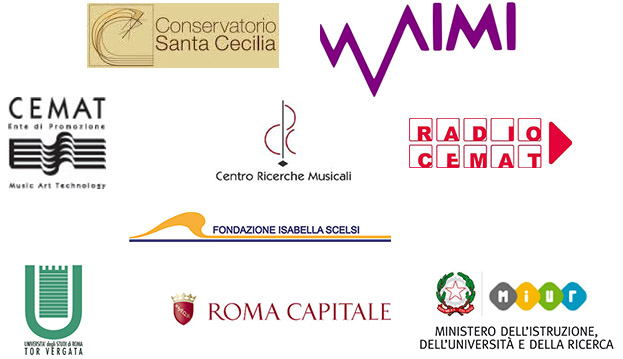
\includegraphics[width=6.4cm]{loghi.jpg}
%%\caption{}
%%\label{fig2_42}
%\end{figure}

\end{document}
